\begin{frame}{Introduction}
    \begin{itemize}
        \item Game ranking data: 24 players play 134 poker games. For each game, there is a ranking for the participants;
        \item Plackett-Luce model for multiple players, generalization of Bradley-Terry model for two players, likelihood, and choice of prior;
        \item Apply MCMC for Bayesian inference on this dataset;
        \item In particular, we want to understand whether the performance of the players depends on two covariates: seniority (age) and skill.
    \end{itemize}
\end{frame}

\begin{frame}{Introduction Ctn.}
    \begin{figure}
        \centering
        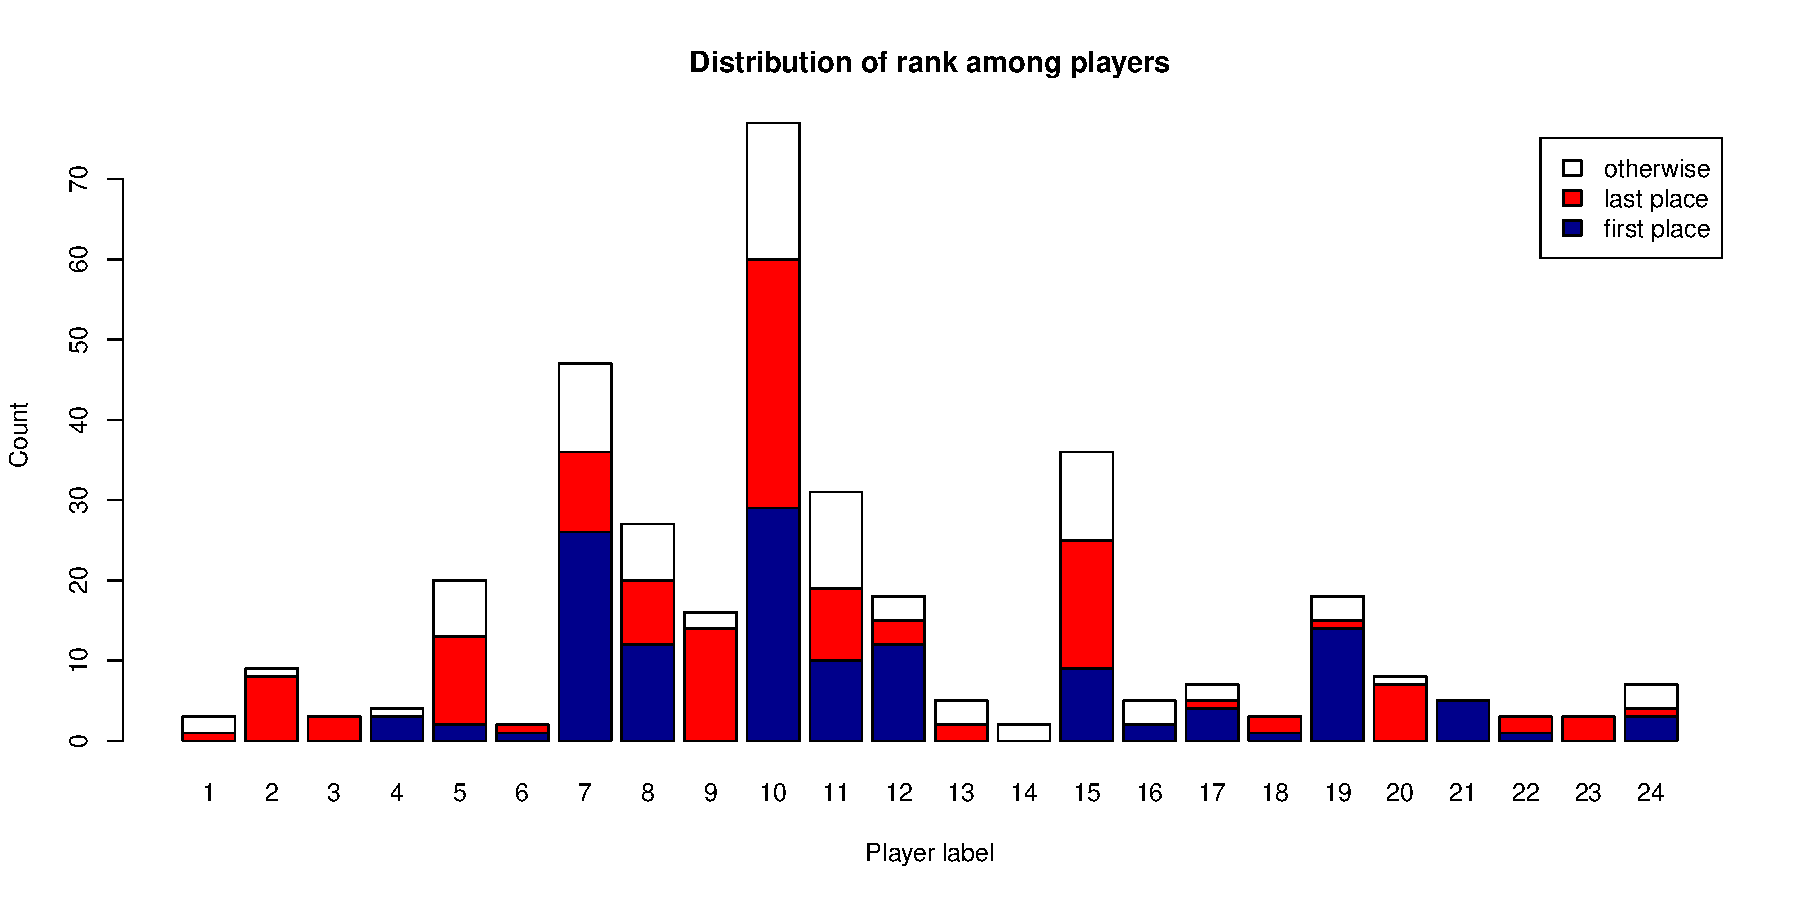
\includegraphics[width=.82\linewidth]{img/player.pdf}
        \caption{The distribution of ranking of the 24 players.}
        \label{fig:players}
    \end{figure}
    \begin{itemize}
        \item Player $10$ takes part in the largest number of games ($77$);
        \item Player $6$ and player $14$ only participate in $2$ games;
        \item Player $19$ has frequency $77\%$ of first place (good player?);
        \item Player $9$ has frequency $87\%$ of last place (bad player?).
    \end{itemize}
\end{frame}

\begin{frame}{Introduction Ctn.}
    \begin{figure}
        \centering
        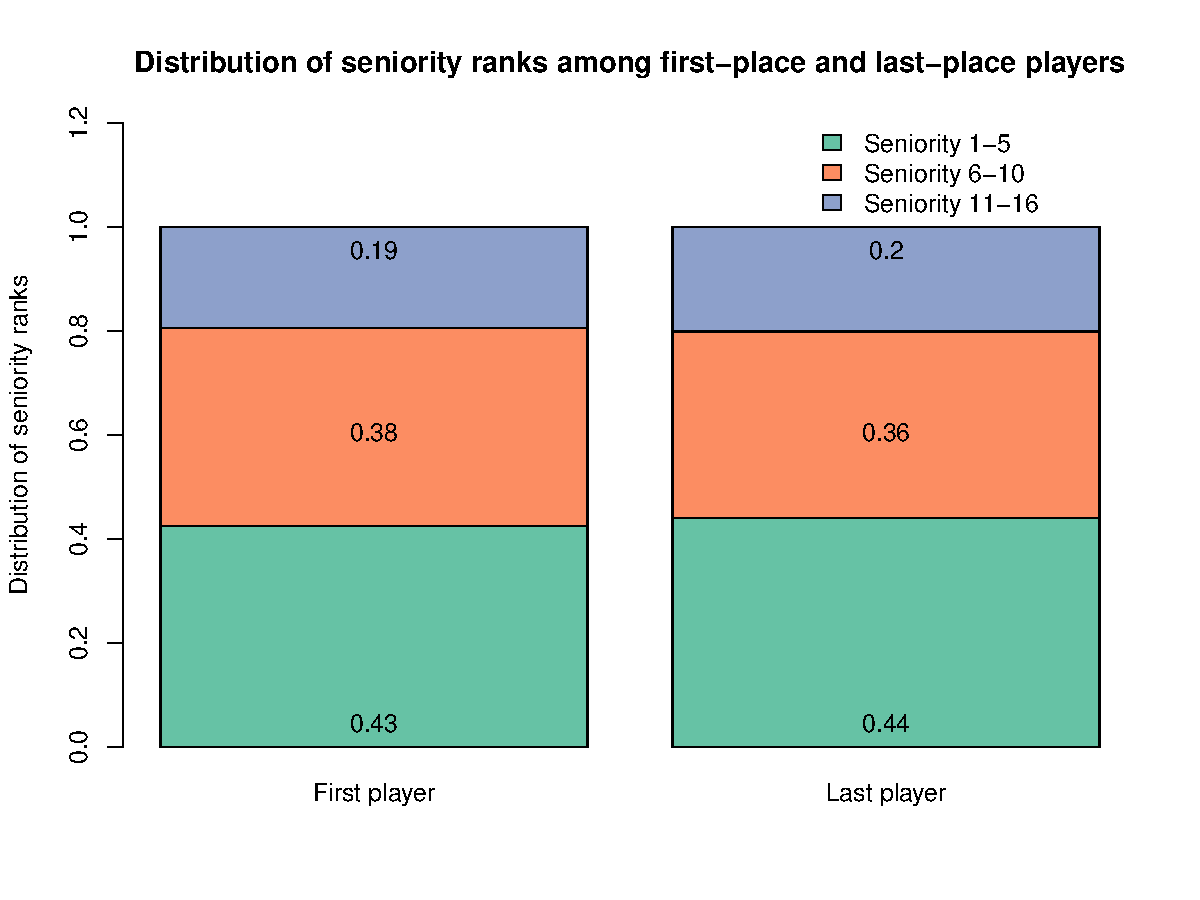
\includegraphics[width=.9\linewidth]{img/seniority.pdf}
        \caption{The distribution of seniority ranks among first-place and last-place players.}
        \label{fig:seniority}
    \end{figure}
\end{frame}
